%---------------------------------------------------------------------
%
%                          Capítulo 2
%
%---------------------------------------------------------------------

\chapter{Marco te'orico}

\section{Antecedentes de la Investigaci'on}

\subsection{Antecedentes Nacionales}

\cite{jrodriguez} publico un articulo denominado ``\emph{Beneficios del modelo As a
service en las pymes}'' cuyo objetivo fue realizar una revisi\'on de conceptos
basicos de la computaci\'on en la nube en especial de los modelos de despliegue
del modelo \emph{As a Service} y algunas consideraciones para su adopci\'on, ventajas
y desventajas llegando a concluir que la computaci\'on en la nube puede ser una
convincente y atractiva forma de adquirir capacidades y reducir los costos; sin
embargo, la peque\~na y mediana empresa necesita acercarse a las implementaciones
en la nube con los ojos abiertos y ser sensibles a algunas cuestiones clave para
asegurar que los beneficios esperados se concreten, las que se presentan a
continuaci\'on:
\begin{enumerate}[a.]
    \item Integraci\'on de las prioridades del negocio y las prioridades de las
          tecnolog\'ias de informaci\'on con la estrategia de despliegue de la
          nube, es decir, los objetivos estrat\'egicos de la empresa o de la
          unidad de negocio necesitan estar claros y entendidos, y a su vez ser
          soportados por la tecnolog\'ia.
    \item Maximizaci\'on en la flexibilidad y agilidad de los negocios
          relacionados con la computaci\'on en nube para un impacto m\'aximo.
          El beneficio real de la cloud computing es su papel potencialmente
          transformador, proporcionando acceso a los recursos consistentes en
          toda la organizaci\'on, con certeza y en forma oportuna.
    \item Disponibilidad 24x7, y crecimiento de la soluci\'on desplegada gracias
          a la alta escalabilidad en el modelo.
    \item La integraci\'on de los recursos de la nube y lo existente fuera de
          ella es a largo plazo; con ello se busca que las empresas puedan agilizar
          sus procesos vitales y de negocio a trav\'es del soporte tecnol\'ogico,
          lo cual a la vez le dar\'a una ventaja competitiva. Con el tiempo, sin
          embargo, las peque\~nas empresas deber\'ian anticipar y alentar este
          desarrollo para el aprovechamiento de los recursos locales y la maximizaci\'on
          de beneficios dirigidos al crecimiento de su negocio.
\end{enumerate}

El articulo en menci\'on servir\'a como gu\'ia para la difusi\'on de estas herramientas
y sus ventajas a los empresarios, as\'i como usar los criterios de selecci\'on
sugeridos para seleccionar las herramientas de computaci\'on en la nube m\'as
adecuadas.

El segundo trabajo de investigaci\'on que se tomo como antecedente lo realizo
\citep{jcampos} quien desarrollo el trabajo denominado ``\emph{INFORM\'ATICA EN LA NUBE
COMO ALTERNATIVA DE ACCESO A LA TECNOLOG\'IA POR PARTE DE LA PEQUE\~NA EMPRESA
OLN S.A}.'', cuyo objetivo fue incrementar la productividad del proceso de
administraci\'on de estados de cuenta de naves, del proceso de venta de fletes
mar\'itimos, y del proceso de gesti\'on de TI a trav\'es de la implementaci\'on
de los servicios inform\'aticos en la nube en la empresa OLN, llegando a las
siguientes conclusiones:
\begin{enumerate}[a.]
    \item La adopci\'on del modelo en la nube suscita muchas dudas, aunque es en
          los a\~nos recientes en que ha alcanzado niveles cada vez m\'as amplios
          de difusi\'on y tambi\'en de oferta de servicios, sin embargo vencer la
          resistencia de las peque\~nas empresas como OLN para embarcarse en un
          aventura tecnol\'ogica en la cual la desmaterializaci\'on de la
          infraestructura juega un papel preponderante fue una tarea dif\'icil
          de asumir, primero porque no se tienen a la vista los componentes
          tangibles que albergan los valiosos activos de informaci\'on de la
          empresa y por otro lado porque tampoco se sabe en qu\'e parte del
          planeta estos se encuentran, esto crea una sensaci\'on de desamparo en
          la plana directiva de lo empresa lo cual fue necesario vencer
          pacientemente abogando por el elemento primario que siempre est\'a en
          las consideraciones del propietario y/o gerente de una empresa y esto
          es el aspecto econ\'omico.
    \item Es as\'i que OLN dio el primer paso, t\'imido al principio, de arriesgarse
          a ahondar en el modelo en la nube y del autor de esta tesis de acompa\~narlos
          en la aventura de mostrarles que el modelo en la nube es mucho m\'as
          que una alternativa barata de tercerizaci\'on de servicios. Lo dicho
          anteriormente llev\'o a que el proyecto se extendiera al conjunto de
          los procesos de la empresa y se viera de que forma el nuevo modelo
          pod\'ia incrementar la productividad puntual de los procesos, vistos
          estos de manera ecl\'ectica.
    \item De la idea establecida en la mente de los directivos de OLN en la cual
          toda automatizaci\'on de procesos de\'ia hacerse a la medida con la
          consecuente contrataci\'on de especialistas, equipos, licencias, etc.
          o de lo contrario con la compra de un software ya echo y que deb\'ia
          pasar por un doloroso proceso de personalizaci\'on con la compra tambi\'en
          de licencias, eventualmente de equipos y siempre con la participaci\'on
          de expertos en inform\'atica, se pas\'o de pronto al empleo de aplicaciones
          en la nube listas para ser usadas desde el primer momento y que inclusive
          pod\'ian ser buscadas y encontradas en Internet con la ayuda de los
          mismos interesados sin que mediara ``un equipo de expertos de TI'',
          con la posibilidad adem\'as de usar un periodo de prueba gratuito,
          usualmente de un mes, otorgado por los proveedores
    \item De este modo se alcanz\'o el primer objetivo primario que ten\'ia que
          ver con el aumento de la productividad y que en el caso presente se
          consigui\'o al elevar la productividad del proceso de administraci\'on
          de estados de cuentas de naves elevando la media de estados de cuenta
          procesados por hora hombre de 0.58 a 0.65, sin contar con los beneficios
          intangibles que conlleva el haber aumentado la satisfacci\'on de los
          clientes a los cuales se les brindada este servicio y la aligeraci\'on
          de la carga operativa del personal encargado de esta tarea
    \item El aumento de la productividad tambi\'en se reflej\'o en las ventas de
          fletes mar\'itimos en cuyo caso fue necesario gestionar los cambios en
          el proceso de ventas de manera m\'as ``fina'' en la medida que el personal
          de ventas, bajo el esquema anterior a la adopci\'on del modelo en la
          nube, operaba cada uno como un compartimento estanco en donde cada
          integrante del equipo de ventas ten\'ia sus clientes (no de la empresa
          sino que los consideraban suyos a t\'itulo personal de modo que si se
          iban de la empresa se llevaban a sus clientes ) y operaba de manera
          m\'as o menos independiente. Vencida la resistencia al cambio, entre
          otras cosas, con la incorporaci\'on intencional del gerente de ventas
          al equipo del proyecto de modo que este actuara adem\'as como catalizador
          de las reacciones de sus subordinados y del apoyo expl\'icito al
          proyecto manifestado personalmente por el gerente general y propietario
          de la empresa.
    \item Se automatiz\'o la administraci\'on del proceso de ventas de fletes y
          como consecuencia se obtuvo un incremento en las ventas de 12\% con
          respecto al periodo anterior. Nuevamente en este caso la manifestaci\'on
          tangible de beneficio se da por el porcentaje de incremento en las ventas,
          sin embargo se obtuvieron otros beneficios menos evidentes como la
          recolecci\'on de m\'etricas diversas sobre todo el proceso de ventas,
          la centralizaci\'on de la informaci\'on de los clientes, de modo que
          estos dejaron de ser propiedad de los representantes comerciales para
          pasar a ser clientes de la empresa, la disponibilidad de m\'ultiples
          an\'alisis provistos de manera autom\'atica por la aplicaci\'on y algo
          muy importante, la adopci\'on de las mejores pr\'acticas para el proceso
          de ventas las cuales vienen ya incorporadas en la soluci\'on adoptada.
    \item En un nivel m\'as bajo de la adopci\'on del modelo en la nube que es
          el que corresponde a la infraestructura como servicio (IaaS) y la
          plataforma como servicio (PaaS) tambi\'en se obtuvieron beneficios
          relevantes, de car\'acter econ\'omico en primer lugar pero tambi\'en
          al nivel operativo puesto el proceso de atenci\'on de las necesidades
          de especializadas de TI pas\'o de ser b\'asicamente presencial a
          mayoritariamente remoto adem\'as de reducir dr\'asticamente el empleo
          de ciertos especialistas y de simplificar tremendamente la administraci\'on
          de TI y liberando el espacio f\'isico que otrora fuera ocupado por la
          infraestructura de TI.
    \item Lo anterior tiene que ver con el segundo objetivo secundario de este
          trabajo que consisti\'o en aumentar la productividad del proceso de
          gesti\'on de TI con respecto al costo de adquisici\'on lo cual dio como
          resultado que bajo el modelo convencional se procesaron 31.60 transacciones
          por cada d\'olar invertido durante el periodo pre test, mientras que
          bajo el modelo en la nube la cantidad de transacciones por d\'olar
          aumenta a 348.54 es decir el costo por transacci\'on durante el post
          test es 1,003\% m\'as bajo que el pretest.
    \item En lo referente a la productividad de TI con respecto a las horas
          hombre de soporte se ha arribado a un resultado positivo al corroborarse
          que en el que en el periodo pre-test se empleaba una hora hombre por
          cada 479 transacciones realizadas, mientras que en post test este valor
          ascendi\'o a 1,101 transacciones por hora hombre empleada en dar
          mantenimiento a TI, lo cual verifica que el incremento del post test
          fue de 130\% con respecto al pre test.
    \item Lo anterior es un hecho y est\'a comprobado se nos quedan, sin embargo,
          en el tintero otros aspectos que no alcanzamos a medir por la premura
          del tiempo o por la dificultad de su realizaci\'on, es as\'i que los
          beneficios de la adopci\'on de la ofim\'atica en la nube no est\'an
          suficientemente representados en los resultados puesto que no se han
          medido innovaciones tales como el trabajo colaborativo en donde muchos
          usuarios trabajan simult\'aneamente en un mismo documento sin importar
          el lugar del mundo en donde est\'en o el dispositivo que est\'en empleando,
          empleando simult\'aneamente herramientas como comunicaci\'on de audio,
          video, mensajer\'ia instant\'anea y otras herramientas m\'as que no
          viene al caso enumerar. De manera tangencial ha surgido de manera embrionaria
          un atisbo de teletrabajo puesto que ahora todos los usuarios tiene tanto
          su mensajer\'ia como sus documentos en la nube, de modo que es
          indiferente el lugar geogr\'afico desde donde los acceden adem\'as,
          de poder compartirlos a voluntad tanto al interior como al exterior de
          la empresa de modo que ha disminuido la presi\'on por estar siempre
          presente en la oficina. Lo mencionado constituye de por si innovaciones
          pero a su vez estos nuevos m\'etodos de trabajo abren las puertas para
          que nazcan nuevas innovaciones suscitadas por el devenir del empleo de
          las herramientas tratadas l\'ineas arriba.
    \item Se ha mencionado anteriormente que la infraestructura de TI fue llevada
          a la nube lo cual comport\'o un ahorro fundamentalmente econ\'omico,
          pero existe otra faceta, nuevamente dif\'icil de medir, pero que tiene
          un potencial muy grande, esto es que en el esquema tradicional la
          capacidad de TI estaba constre\~nida a las limitaciones f\'isicas de los
          equipos que pose\'ia la empresa y cualquier ampliaci\'on resultaba
          costosa en tiempo y dinero, mientras que bajo el modelo en la nube
          los l\'imites han desaparecido, la capacidad de procesamiento de OLN
          se ha tornado virtualmente infinita y aun as\'i sin que se tenga que
          incurrir en grandes inversiones y esperas.
    \item Lo dicho en el p\'arrafo anterior a potenciado las posibilidades de OLN
          puesto que puede responder a exigencias en cuanto a sofisticaci\'on
          tecnol\'ogica de ciertos clientes transnacionales, lo cual lo pone en
          posici\'on de competir con empresas de mucha mayor envergadura sin
          contar con que ahora cuenta con los recursos para montar una infraestructura
          de TI compleja para probar o demostrar alg\'un producto o servicio (esto
          se da por ejemplo cuando se participa en una licitaci\'on en donde se
          debe estar en capacidad de operar alg\'un proceso automatizado poco
          despu\'es de haber ganado la buena pro) y luego desmontarla r\'apidamente
          con poca esfuerzo y sin inversiones de capital.
\end{enumerate}

El trabajo mencionado servir\'a como referencia para la elaboraci\'on de los instrumentos
de medici\'on ya que se trata de un caso muy similar al presente trabajo pero limitado
a una sola empresa.

%-----------------
\subsection{Antecedentes Internacionales}

\cite{diaz} desarroll\'o el trabajo ``\emph{EL CLOUD COMPUTING EN LA PYME ESPA\~NOLA}''
con el objetivo de analizar las posibilidades de uno de los productos de la empresa
Intelligence Partner, que consiste en una aplicación de gestión de activos inmobiliarios, y
para ello se puso en contexto el entorno de las Pymes y más en concreto el
sector inmobiliario español con la intención de ver las posibilidades de venta
que tiene esta aplicación en la nube, llegando a concluir que a pesar beneficios
destacados a lo largo de todo el documento, el cloud computing es una tecnología
relativamente nueva. Hay varias cuestiones que deben tenerse en cuenta antes cambiar
todos los sistemas tradicionales de la pequeña empresa por la computación en la nube.
A continuación presentamos algunos aspectos que deben considerarse antes de que una
empresa decida adaptar sus sistemas a la nube:
\begin{itemize}
    \item Es importante tener un profundo conocimiento de la infraestructura de TI
            existente. Se recomienda a las empresas tener en cuenta cuatro puntos
            antes de tomar una decisión, el tamaño de las infraestructuras de TI, los
            patrones de uso, la sensibilidad de los datos y lo importante que son las
            operaciones informáticas para la empresa.
    \item Muchos analistas han señalado el problema del monopolio a la hora de
            ofrecer servicios de cloud computing. La cuestión de la dependencia de
            un proveedor puede tener graves repercusiones para las pequeñas
            empresas en caso de pérdida de datos. A medida que los servicios se
            ofrecen a través de software propietario y la falta de normas hace de la
            portabilidad de una de las principales preocupaciones.
    \item Se espera que la nube maneje una gran cantidad de datos. Por lo tanto,
            es importante entender las cuestiones clave en cuanto a la seguridad y
            los riesgos potenciales. La revisión de los protocolos de seguridad en
            varios modelos de cloud revela la necesidad de un marco estandarizado.
            Por ejemplo, con SaaS, una de las principales preocupaciones es la falta
            de control y la total dependencia del proveedor para garantizar las
            medidas de seguridad adecuadas. Otra cuestión es garantizar la
            seguridad, la integridad y la persistencia de los datos durante la
            transferencia de datos dentro y el mantenimiento de la confidencialidad
            de los datos de los clientes
\end{itemize}

Este trabajo servir\'a para elaborar el dise\~no operativo concreto para la implementaci\'on
de cada herramienta en las MiPYME del Centro de Desarrollo Empresarial del Cusco.

\cite{Salauddin} desarrollo el trabajo denominado ``\emph{A study on cloud
computing adoption of small and medium enterprises}'' con el objetivo de proveer
una visi\'on de los efectos, riesgos percibidos, requerimientos y beneficios de la
adopci\'on de las herramientas de la computaci\'on en la nube en general. Adem\'as
de investigar los beneficios y oportunidades que los atributos de la computaci\'on
en la nube ofrecen como la flexibilidad, despliegue rapido y en particular los
costos que pueden ayudar a la adopci\'on de estas herramientas. Las conclusiones
obtenidas son las siguientes:

Por otro lado, \citep{brimbela} realizo el trabajo: ``\emph{Adoption of Cloud
Computing by SME'S in Emerging Markets (Brazil)}''

Este es el ultimo \citep{saleem} y este es otro

\section{Bases Te'oricas}

\subsection{Computaci\'on en la nube}

\subsubsection{Definici\'on de Computaci\'on en la nube}
``\emph{Cloud computing es un modelo que permite el acceso bajo demanda y a trav\'es de
la red a un conjunto de recursos compartidos y configurables (como redes,
servidores, capacidad de almacenamiento, aplicaciones y servicios) que pueden
ser r\'apidamente asignados y liberados con una m\'inima gesti\'on por parte del
proveedor del servicio}''\citep{cierco}.

Ya que la computaci\'on en la nube permite el acceso a los recursos bajo demanda,
es decir en el momento que se necesite, tambi\'en es factible que estos servicios
sean cobrados seg\'un el tiempo de uso de los mismos de forma transparente y fiable.

Tambi\'en permite la expansi\'on o reducci\'on de las capacidades de estos
recursos segun la necesidad del momento de las aplicaciones o servicios, a lo
que le llama ``Elasticidad''.

\subsubsection{Caracteristicas fundamentales de la Computaci\'on en la Nube}
\cite{nist} indican que las caracter\'isticas fundamentales necesarias para poder
mantener un modelo de computo en la nube comprenden:
\begin{itemize}
    \item \textbf{Autoservicio bajo demanda.-} La tecnolog\'ia en la nube
          proporciona recursos de una forma automatizada los usuarios pueden
          agregar o quitar servicios basados en sus necesidades y requerimientos
          del negocio.
    \item \textbf{Elasticidad rapida.-} Consiste en dotar a un servicio de mayores
          recursos de computo para cubrir sus necesidades y as\'i mismo regresar
          a estados anteriores cuando ya no requiera de estos recursos.
    \item \textbf{Agrupaci\'on de recursos.-} La arquitectura de la nube tiene la capacidad
          de creaci\'on de recursos compartidos que hacen que la nube sea
          econ\'omicamente viable.
    \item \textbf{Facturaci\'on y m\'etricas de uso de servicio.-} Los usuarios
          pagan por los recursos que han contratado o por el uso de recursos, y
          los entornos de cloud computing deben de incluir mecanismos de monitoreo
          de uso de recursos para la facturaci\'on y/o mejora del servicio.
    \item \textbf{Amplio acceso a la red.-} Las capacidades est\'an disponibles
          a trav\'es de la red y se accede a trav\'es de mecanismos est\'andar
          que promueven el uso de plataformas de clientes finas o gruesas
          heterog\'eneas (por ejemplo, tel\'efonos m\'oviles, tablets, port\'atiles
          y estaciones de trabajo).
\end{itemize}
%--------------------------------------------------
\subsubsection{Tipos de nubes por el modelo de despliegue.}
\cite{nist} indican que los tipos de nubes por el modelo de despliegue son:
\begin{enumerate}
    \item \textbf{Nube privada}, en  la  que  los  servicios  cloud  no  son
          ofrecidos  al  p\'ublico  en  general. Pueden distinguirse a su vez dos
          situaciones:
          \begin{enumerate}[a.]
              \item \textbf{Cloud propia}. La infraestructura es \'entegramente gestionada
                    por una organizaci\'on.
              \item \textbf{Cloud compartida}. La  infraestructura  es  compartida  por
                    varias organizaciones.
          \end{enumerate}
    \item \textbf{Cloud p\'iublica}. La  infraestructura  es  operada  por  un
          proveedor  que  ofrece  servicios al p\'iublico en general.
    \item \textbf{Cloud h\'ibrida}. Resultado de la combinaci\'on de dos o m\'as clouds
          individuales que, pudiendo ser a su vez propias, compartidas o p\'iblicas,
          permite portar datos o aplicaciones entre ellas.
\end{enumerate}

\begin{figure}[h]
    \centering
    \captionsetup{justification=centering}
    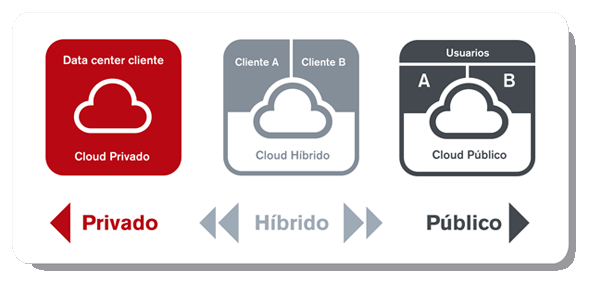
\includegraphics[width=0.7\textwidth]{Imagenes/Bitmap/cloud0}
    \caption{Modelos de despliegue de la computaci\'on en la nube}
    \label{fig:cloud1}
\end{figure}

\subsubsection{Tipos de nubes por el modelo de servicio}
Seg\'un \cite{nist} se ofrecen tres modelos de servicio:
\begin{enumerate}
    \item \textbf{Software as a Service - SaaS}.- Al usuario se le ofrece la
          capacidad de que las aplicaciones  que  su  proveedor  le  suministra
          corran  en  una  infraestructura cloud, siendo las aplicaciones accesibles
          a trav\'es de, por ejemplo, un navegador web como en el caso del webmail,
          que es posiblemente el ejemplo m\'as representativo, por lo extendido,
          de este modelo de servicio. El usuario carece de cualquier control sobre
          la infraestructura o sobre las propias aplicaciones, excepci\'on hecha
          de las posibles configuraciones de usuario o personalizaciones que se
          le permitan.
    \item \textbf{Platform as a Service}.- Al usuario se le permite desplegar
          aplicaciones propias  (ya  sean  adquiridas  o  desarrolladas  por  el
          propio  usuario)  en  la  infraestructura cloud de  su  proveedor, que
          es  quien  ofrece  la  plataforma  de desarrollo y las herramientas de
          programaci\'on. En este caso, es el usuario quien mantiene el control de
          la aplicaci\'on, aunque no de toda la infraestructura subyacente.
    \item \textbf{Infrastructure as a Service}.- El proveedor ofrece al usuario
          recursos como capacidad  de  procesamiento,  de  almacenamiento,  o
          comunicaciones, que el usuario puede utilizar para ejecutar cualquier
          tipo de software, desde sistemas operativos hasta aplicaciones.
\end{enumerate}

\begin{figure}[h]
    \centering
    \captionsetup{justification=centering}
    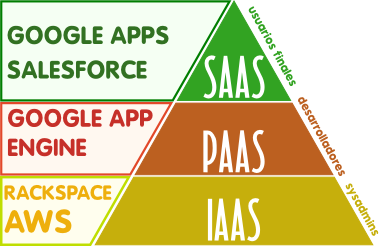
\includegraphics[width=0.7\textwidth]{Imagenes/Bitmap/cloud1}
    \caption{Modelos de servicio de la computaci\'on en la nube con algunos proveedores en cada tipo.}
    \label{fig:cloud1}
\end{figure}

\subsubsection{Beneficios de la computaci\'on en la nube}
``\emph{Los beneficios del cloud son muy relevantes desde distintos puntos de vista.
Para la econom\'ia global, el traslado de las econom\'ias de escala de los
proveedores a las empresas usuarias reduce los costes globales en TI, elimina
las barreras de entrada para nuevos actores y dinamiza la econom\'ia, promoviendo
la aparici\'on de nuevos modelos de negocio y lineas de actividad, facilitando
por la creaci\'on de empresas y de empleo}''\citep{cierco}.

%\subsection{Definici'on conceptual}

%\subsection{Definici'on operacional}

\section{Hip'otesis}

\subsection{Hip'otesis General}

Existe un efecto positivo del uso de la computaci\'on en la nube en la
gesti'on de las micro, peque\~nas y medianas empresas pertenecientes al Centro de
Desarrollo Empresarial del Cusco.

\subsection{Hip'otesis Espec'ificas}
\begin{enumerate}[a.]
    % preguntaar si es necesario colocar las palabras pe-post implementacion
    \item El nivel de gesti\'on de las MiPYMES pertenecientes al Centro de Desarrollo
          Empresarial del Cusco antes del uso de las herramientas de la computaci\'on
          en la nube es deficiente.
    \item El nivel de gesti\'on de las MiPYMES pertenecientes al Centro de Desarrollo
          Empresarial del Cusco despu\'es del uso de las herramientas de la computaci\'on
          en la nube es eficiente.
    \item El efecto del uso de herramientas de la computaci'on en la nube en la
          gesti\'on de las MiPYMES pertenecientes al Centro de Desarrollo Empresarial
          del Cusco es positiva.
\end{enumerate}

\section{Variables}

\subsection{Identificaci'on de variables}

\begin{enumerate}[a.]
    \item Uso de herramientas de computaci\'on en la nube.
    \item Gesti\'on Empresarial.
\end{enumerate}

\subsection{Operacionalizaci'on de variables}
%-----------------
\begin{table}[htbp]
    \caption{Operacionalizaci\'on de variables}
    \label{t_sim}
    \centering
        \begin{tabular}{|p{3cm}|p{2cm}|p{2cm}|p{3cm}|p{3cm}|}
            \hline
            \thead{Variables} & \thead{Definici\'on \\ Conceptual} & \thead{Definici\'on \\ Operacional} & \thead{Dimensiones} & \thead{Indicadores} \\ \hline
            % Primera fila
            Uso de herramientas de computaci\'on en la nube &
            \emph{trabajo en progreso} &
            \emph{trabajo en progreso} &
            \emph{trabajo en progreso} &
            \emph{trabajo en progreso} \\
            \hline
            % Segunda fila
            Gesti\'on Empresarial &
            \emph{trabajo en progreso} &
            \emph{trabajo en progreso} &
            \emph{trabajo en progreso} &
            \emph{trabajo en progreso} \\
            \hline
        \end{tabular}
        Fuente: Elaboraci\'on propia.
\end{table}
%-----------------
\section{Definici'on de t'erminos b'asicos}
